% LaTeX path to the root directory of the current project
\providecommand{\econtexRoot}{}
\renewcommand{\econtexRoot}{..}
\providecommand{\econtexPaths}{LaTeX}\renewcommand{\econtexPaths}{\econtexRoot/LaTeX/econtexPaths}
\documentclass{econtex}
% LaTeX path to the root directory of the current project
\providecommand{\econtexRoot}{}
\renewcommand{\econtexRoot}{..}
\providecommand{\econtexPaths}{LaTeX}\renewcommand{\econtexPaths}{\econtexRoot/LaTeX/econtexPaths}
%\input{\LaTeXFiles/econtex_onlyinsubfile}
%\onlyinsubfile{\externaldocument{\LaTeXFiles/BufferStockTheory}}
\usepackage{\LaTeXFiles/BufferStockTheory}
\newcommand{\BSTlinkTo}{https://\owner.github.io/BufferStockTheory}
\renewcommand{\FHWC}{\href{{\BSTlinkTo}FHWC}{\textrm{FHWC}}}
\newcommand{\FHWCFull}{\href{{\BSTlinkTo}\#FHWC}{{\BSTlinkTo}\#FHWC}}
\newcommand{\PFGICFull}{\href{{\BSTlinkTo}\#PFGIC}{{\BSTlinkTo}\#PFGIC}}
\newcommand{\RICFull}{\href{{\BSTlinkTo}\#RIC}{{\BSTlinkTo}\#RIC}}
\newcommand{\PFFVACFull}{\href{{\BSTlinkTo}\#PFFVAC}{{\BSTlinkTo}\#RIC}}
\renewcommand{\FHWC}{\href{{\BSTlinkTo}\#FHWC}{\textrm{FHWC}}}
\renewcommand{\PFGIC}{\href{{\BSTlinkTo}\#PFGIC}{\textrm{PF-GIC}}}
\renewcommand{\RIC}{\href{{\BSTlinkTo}\#RIC}{\textrm{RIC}}}
\renewcommand{\PFFVAC}{\href{{\BSTlinkTo}\#PFFVAC}{\textrm{PF-FVAC}}}

\begin{document}

\hypertarget{ApndxConditionDiagrams}{}

\section{Relational Diagrams for the Inequality Conditions}\label{sec:ApndxConDia}

This appendix explains in detail the paper's `inequalities' diagrams (Figures~\ref{fig:RelatePFGICFHWCRICPFFVAC},\ref{fig:Inequalities}).

\hypertarget{InequalityPFGICFHWCRIC}{}
\begin{figure}
\centering
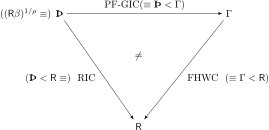
\includegraphics[width=4in]{\FigDir/InequalityPFGICFHWCRIC}
\caption{Inequality Conditions for Perfect Foresight Model}
\centerline{ (Start at a node and follow arrows)}
\label{fig:InequalityPFGICFHWCRIC}
\end{figure}

\end{document}
